\documentclass[a4paper,12pt]{article}
\usepackage{amssymb}
\usepackage{amsfonts}

% Кодировка и язык
\usepackage[utf8]{inputenc}
\usepackage[T2A]{fontenc}
\usepackage[russian]{babel}


% Математические пакеты
\usepackage{amsmath,amsfonts,amssymb}
%Таблицы
\usepackage{array}
\usepackage{booktabs} % Для более красивых горизонтальных линий в таблицах
\usepackage{graphicx}
\usepackage{array}
\usepackage{booktabs}
% Геометрия страницы
\usepackage{geometry}
\geometry{top=2cm, bottom=2cm, left=2.5cm, right=2.5cm}
% Гиперссылки (лучше загружать последним)
\usepackage{hyperref}


% Настройки заголовка
\title{Домашнее задание}
\author{Студент: \textbf{Ростислав Лохов}}
\date{\today}

\begin{document}

% Титульный лист
\begin{titlepage}
    \centering
    \vspace*{1cm}

    \Huge
    \textbf{Домашнее задание}

    \vspace{0.5cm}
    \LARGE
    По курсу: \textbf{Экономика}

    \vspace{1.5cm}

    \textbf{Студент: Ростислав Лохов}

    \vfill

    \Large
    АНО ВО Центральный университет\\
    \vspace{0.3cm}
    \today

\end{titlepage}

% Содержание
\tableofcontents
\newpage

% Основной текст
\section{Сине-Красный уровень}


\subsection{Задача 1}
\begin{enumerate}
    \item Излишек продавцов - 800. Излишек покупателей - 800. Общественное благосостояние - 1600.
    \item Излишек покупателей - 1050. Излишек продавцов - 450. Общественное благосостояние - 1500. Мертвый груз - 100. 
\end{enumerate}

\subsection{Задача 2}
\begin{enumerate}
    \item кривая предложения повышается на константу 
    \item кривые не будут сходится, т.е будет просто разрыв, они будут ограничены количеством
    \item график вернется в изначальную позицию
\end{enumerate}
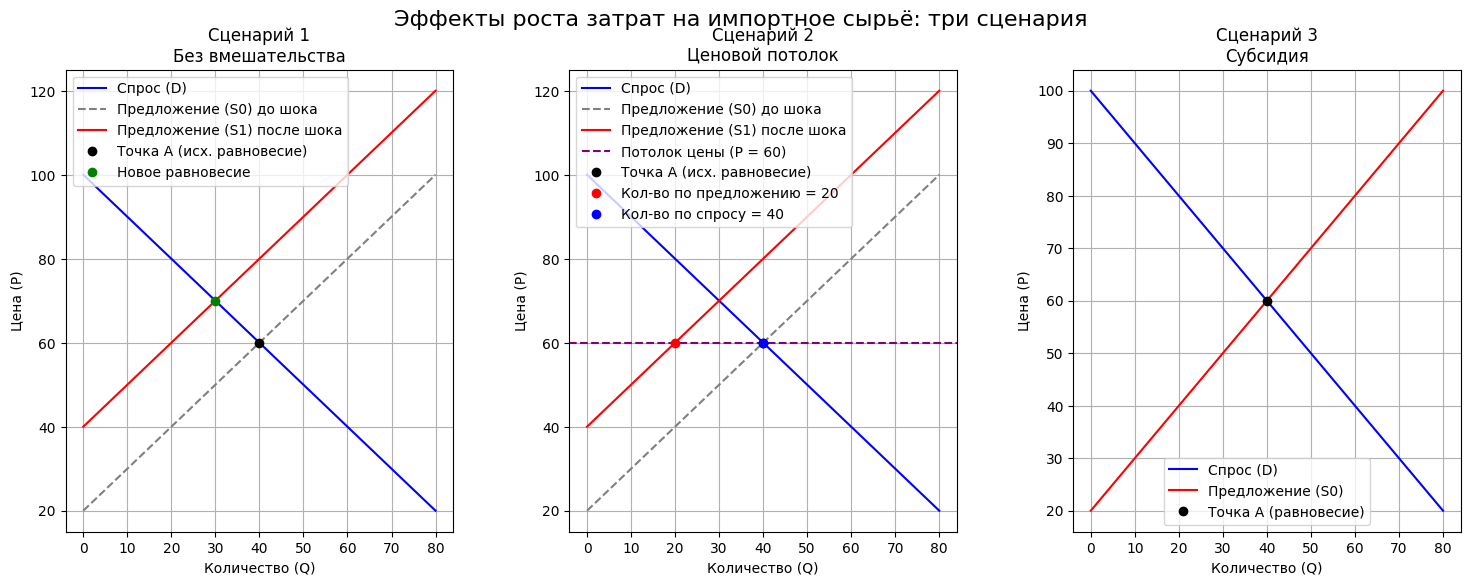
\includegraphics[scale=0.4]{graphs/3.1.png}
\begin{enumerate}
    \item Сценарий 3 т.к стоимость не повысится
    \item Достоинства - В, Г, Д
    \item Недостатки - А, Б, Е
\end{enumerate}

\subsection{Задача 3}
\begin{enumerate}
    \item Наличие Армии. Защита от внешней агрессии одного армией не уменьшает уровень защиты армией для всех других граждан. Невозможно не охранять какого-то гражданина. Все граждане получают выгоду от этого.
    \item Курение сигарет в общественном мест. человек курящий сигарету распространяет выдыхаемый дым на других, что негативно влияет на их здоровье.
    \item Производство вакцин. Вакцинируя одних мы разрываем цепочки заражения, тем самым уменьшаем количество болеющих.
\end{enumerate}

\subsection{Задача 4}
\begin{enumerate}
    \item Равновесная цена - 30. 
    \item Обьем продаж - 200.
    \item Избытки потребителя - 2000. 
    \item Избытки покупателя - 2000. 
    \item Общественное благосостояние - 4000. 
\end{enumerate}

\begin{enumerate}
    \item Равновесная цена изменилась до 20, Обьем продаж упадет вдвое, Избытки потребителя - 2500, Избытки производителя - 500, Общественное благосостояние - 3000. Мертвый груз - 1000
    \item Равновесная цена увеличилась до 40, Обьем продаж упадет вдвое, Избытки потребителя - 500, Избытки производителя - 2500, Общественное благосостояние - 3000. Мертвый груз - 1000
    \item Равновесная цена увеличилась до 35, Обьем продаж упадет до 150, Избытки потребителя - 1125, Избытки производителя - 1125, Избытки гос-ва 1500, Общественное благосостояние - 3750. Мертвый груз - 250
    \item Равновесная цена увеличилась до 25, Обьем продаж упадет до 250, Избытки потребителя - 3125, Избытки производителя - 3125, Избытки гос-ва -2500, Общественное благосостояние - 3750. Мертвый груз - 250
    \item Равновесная цена увеличилась до 25, Обьем продаж упадет до 250, Избытки потребителя - 3125, Избытки производителя - 3125, Избытки гос-ва -2500, Общественное благосостояние - 3750. Мертвый груз - 250
    \item Равновесная цена увеличилась до 35, Обьем продаж упадет до 250, Избытки потребителя - 3125, Избытки производителя - 3125, Избытки гос-ва -2500, Общественное благосостояние - 3750. Мертвый груз - 250
\end{enumerate}

\section{Черный уровень}
\subsection{Задача 1}
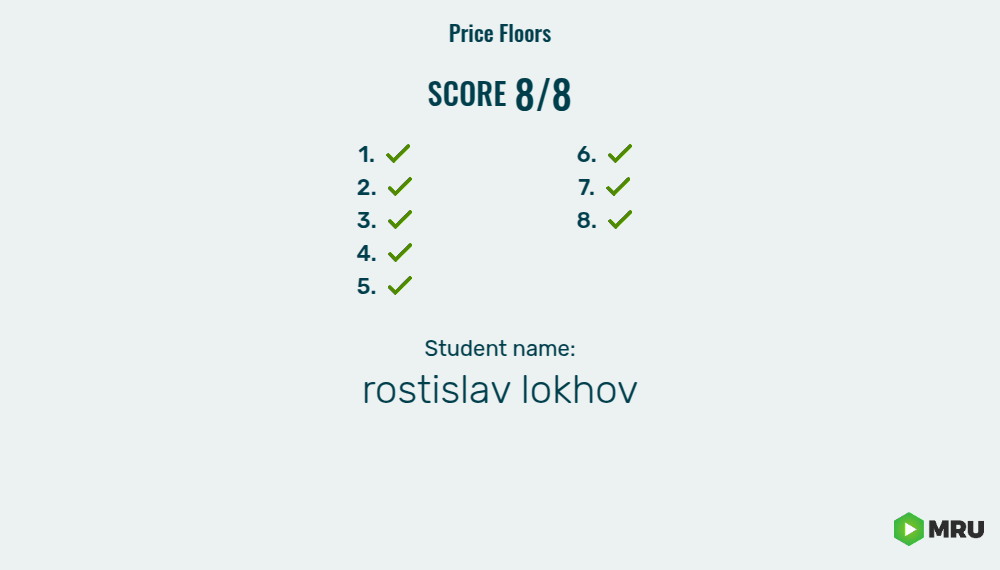
\includegraphics[scale=0.15]{graphs/3.2.jpg}
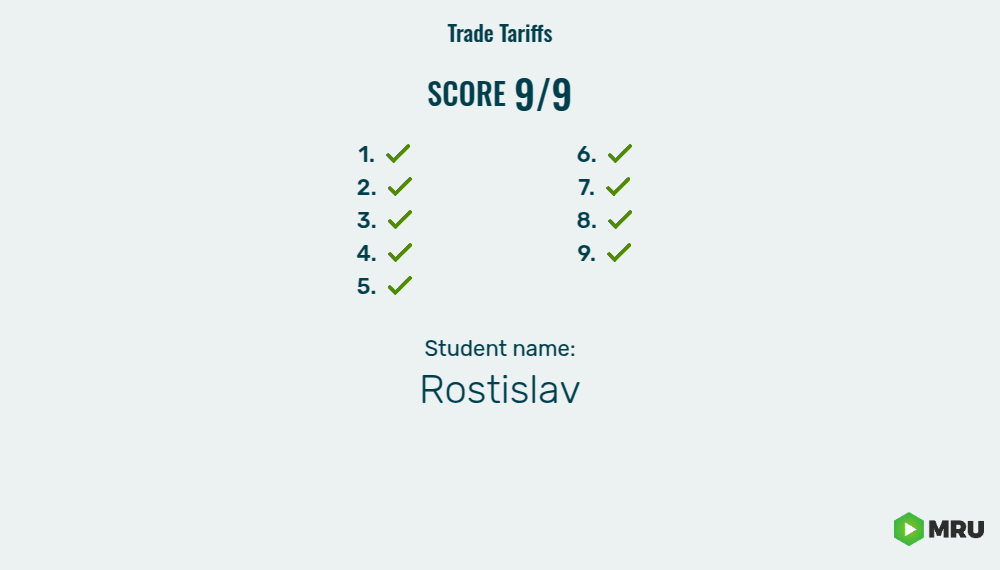
\includegraphics[scale=0.15]{graphs/3.3.jpg}
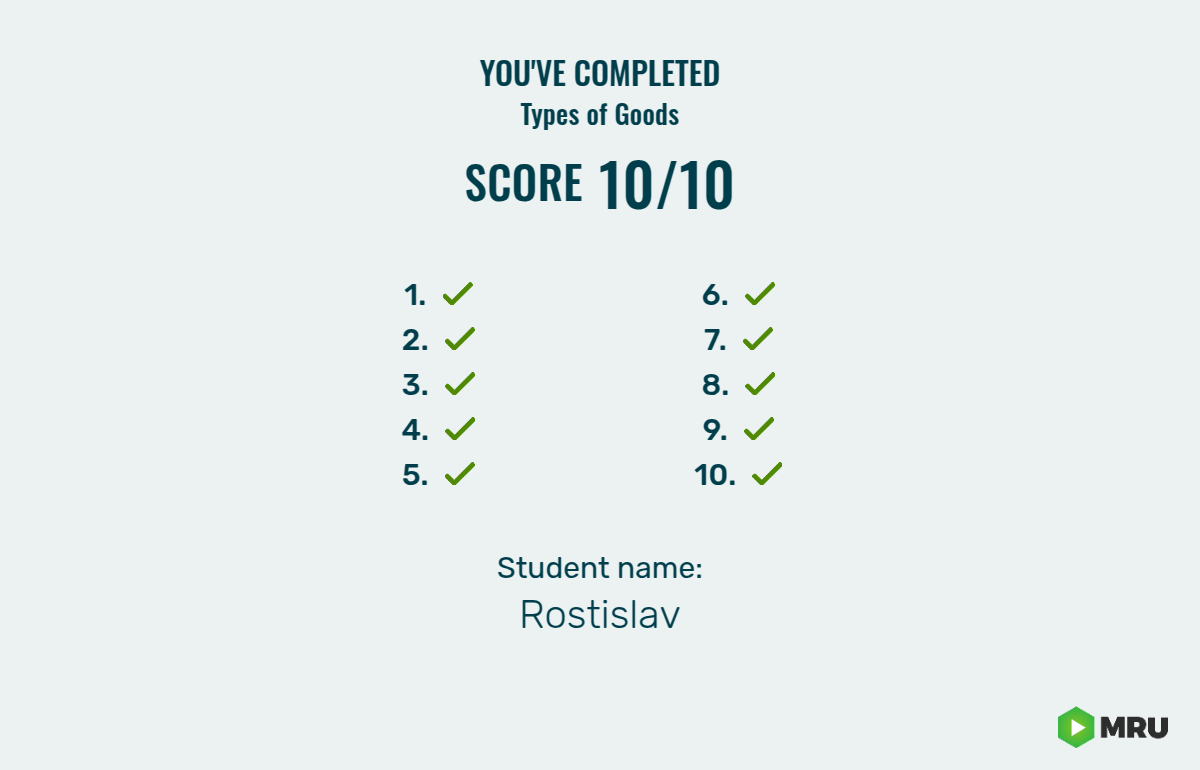
\includegraphics[scale=0.1]{graphs/3.4.jpg}

\subsection{Задача 2}
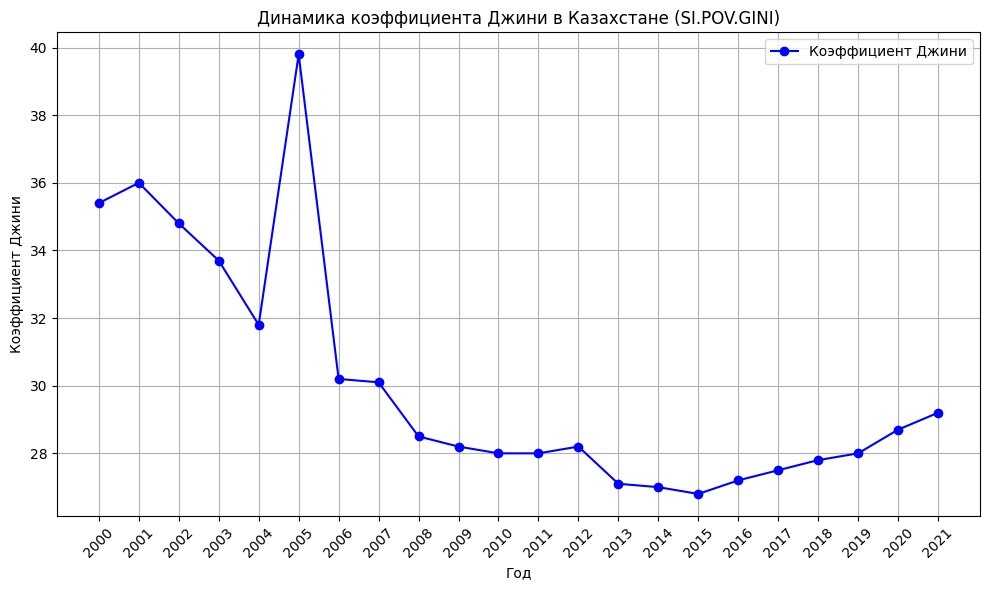
\includegraphics[scale=0.6]{graphs/3.5.png}

На протяжении всего периода в Казахстане наблюдалась положительная динамика в сторону равенства доходов населения. Скачок - скорее всего выброс из за смены методологии расчетов коэффициента джинни

\subsection{Задача 3}
\[
P=20-2Q
\]

\[
P_b = 1.1P
\]

\[
P_b=1.1(20-2Q) = 22-2.2Q
\]

\subsection{Задача 4}
В системе где чаевые сдаются в общий котел, а потом сдаются поровну существует возможность ничего не делать и получать примерно такую же долю. Тем самым больше провоцирует оппортунистическое поведение и проблему безбилетника.

\begin{enumerate}
    \item Преимущества индивидуального распределения: усилия=вознаграждения; Недостатки: конкуренция и разные зоны обслуживания(разные доходы)
    \item Преимущества коллективного распределения: командная работа, сглаживание разницы; Недостатки: проблема безбилетника, отсутствие мотивации.
    \item Для барменов лучше индивидуальное распределение т.к работа на баре подразумевает контакт с клиентами. Официанты - коллективно, т.к обслуживание зала - командная работа
\end{enumerate}

\end{document}